\subsection*{Problem 1}
Prove that if $G$ is a graph on $11$ vertices then at least one of $G$ and its complementary graph $\overline{G}$ is not planar. 

\begin{proof}
We proceed by contradiction. Assume that both $G$ and its complement $\overline{G}$ are planar graphs. Let $n = 11$ be the number of vertices and let $m$ be the number of edges in $G$. The number of edges in the complement $\overline{G}$ is the total number of possible edges in $K_{11}$ minus $m$, so $ |E(\overline{G})| = \binom{11}{2} - m = 55 - m $. Now, note that for a graph with $n \ge 3$ vertices to be planar, we need that $|E| \le 3n - 6$. Since we assumed that $G$ is planar, we have that $ m \le 3(11) - 6 = 27 $, and since we assumed $\overline{G}$ is planar, we have that  $55 - m \le 3(11) - 6 = 27 $. Now, summing these two inequalities yields $ m + (55 - m) \le 27 + 27 \implies 55 \le 54 $, which is a contradiction. Therefore, the assumption that both graphs are planar must be false, and so at least one of them must be non-planar. Thus, if $G$ is a graph on $11$ vertices then at least one of $G$ and its complementary graph $\overline{G}$ is not planar. 
\end{proof}

\subsection*{Problem 2}
What is the minimum number of edge crossings with which the graph $K_{4,4}$ can be drawn on the plane?

\begin{proof}
Let $c$ be the crossing number of $K_{4,4}$. If we remove $c$ edges from the graph (one edge from each crossing), we get a planar subgraph $G'$. The graph $K_{4,4}$ is a bipartite graph with $n=8$ vertices and $m=16$ edges. The planar subgraph $G'$ will have $m' = 16 - c$ edges. Now, for any bipartite planar graph with $n \ge 3$, the number of edges satisfies $|E| \le 2n - 4 $. If we apply this to $G'$, we have that $ 16 - c \le 2(8) - 4 \implies c \ge 4 $, and so the crossing number is at least 4. Thus, the minimum number of edge crossings with which the graph $K_{4,4}$ can be drawn on the plane is 4.
\end{proof}

\subsection*{Problem 3}
Determine the edge-chromatic number of the $d$-dimensional hypercube $Q_d$, where the vertices of $Q_d$ correspond to the elements of $\{0, 1\}^d$ and two vertices are connected if their Hamming distance is $1$.

\begin{proof}
We will first discuss some properties of the graph $Q_d$. Since vertices correspond to the elements of $\{0, 1\}^d$, we have that $|V(Q_d)|=2^d$, and $|E(Q_d)|=d(2^{d-1})$. We will proceed by induction on $d$. For the base case where $d=1$, the graph $Q_1$ is a single edge, which requires 1 color. Thus, $\chi'(Q_1) = 1$. Now for the inductive step, assume $\chi'(Q_d) = d$. The graph $Q_{d+1}$ consists of two copies of $Q_d$. By the inductive hypothesis, we can color the edges within both copies using $d$ colors. The edges that connect the two copies join each vertex in the first copy to its corresponding vertex in the second. Since these connecting edges are a perfect matching, we can assign all of them a single new color, $d+1$. Thus, we have colored $Q_{d+1}$ with $d+1$ colors. Since every vertex has degree $d+1$, we cannot use fewer colors. Therefore, $\chi'(Q_{d+1}) = d+1$.
\end{proof}

\subsection*{Problem 4}
Prove that $R(3, 3) = 6$, where $R(k, \ell)$ denotes the Ramsey number corresponding to $k$ and $\ell$.

\begin{proof}
We first claim that there exists a coloring $K_5$ with neither a red triangle nor a blue triangle, implying that $R(3,3) > 5$. Consider the following colored $K_5$ with no red triangles or blue triangles.

\begin{center}
    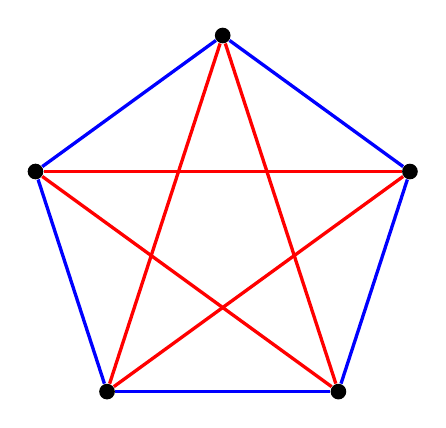
\begin{tikzpicture}[scale=1, every node/.style={circle, fill, inner sep=2pt, draw=none}]
    
        \def\n{5}
        \def\radius{2.5cm}
        \def\startangle{90+360/5}
        \def\step{360/\n}

        \foreach \i in {0,...,4} {%
            \edef\nodename{v\i}%
            \node (\nodename) at ({\startangle - \step*\i}:\radius) {};%
        }

        \draw[blue, very thick] (v0) -- (v1);
        \draw[red, very thick] (v0) -- (v2);
        \draw[red, very thick] (v0) -- (v3);
        \draw[blue, very thick] (v0) -- (v4);

        \draw[blue, very thick] (v1) -- (v2);
        \draw[red, very thick] (v1) -- (v3);
        \draw[red, very thick] (v1) -- (v4);

        \draw[blue, very thick] (v2) -- (v3);
        \draw[red, very thick] (v2) -- (v4);

        \draw[blue, very thick] (v3) -- (v4);
            
    \end{tikzpicture}
\end{center}
Now, we claim that $R(3,3) \leq 6$\footnote{We can prove this easier by considering the fact that $R(k, \ell) \leq R(k, \ell - 1) + R(k-1, \ell)$. Applying the result here yields $R(3, 3) \leq R(3,2) + R(2,3)$. Trivially, we know that $R(2,3) = R(3,2) = 3$, and thus $R(3, 3) \leq 3 + 3 = 6$. However, from the wording of Problem 5, I assume an explicit argument is desired}. Consider a complete graph $K_6$ where every edge is colored either red or blue. We will show that there exists either a red triangle or a blue triangle. First, pick any vertex $v$ in the graph. Since the graph is $K_6$, vertex $v$ is incident to 5 edges. By the Pigeonhole Principle, since there are 5 edges and only 2 colors, at least $\lceil 5/2 \rceil = 3$ edges incident to $v$ must be of the same color. Assume that there are three edges incident to $v$ that are colored blue (without loss of generality) and let the other endpoints of these edges be $u_1, u_2,$ and $u_3$. Consider the edges connecting $u_1, u_2,$ and $u_3$. There are two possible cases, either at least one edge among $\{u_1, u_2, u_3\}$ is blue or none of the edges among $\{u_1, u_2, u_3\}$ are blue. For the first case, suppose the edge $(u_1, u_2)$ is blue. Since the edges $(v, u_1)$ and $(v, u_2)$ are also blue (by our assumption), and so the vertices $\{v, u_1, u_2\}$ form a blue triangle. For the second case, if none of the edges among $\{u_1, u_2, u_3\}$ are blue, then this implies that all edges connecting these vertices must be red, and so the edges $(u_1, u_2)$, $(u_2, u_3)$, and $(u_3, u_1)$ form a red triangle on the vertices $\{u_1, u_2, u_3\}$. In both cases, the graph $K_6$ contains a monochromatic triangle. Thus, $R(3,3) \leq 6$. Since $R(3,3) \leq 6$ and $R(3,3) > 5$, we have that $R(3,3) = 6$

\end{proof}

\subsection*{Problem 5}
Show that $R(4, 3) \leq 10$ by proving that every red/blue coloring of the edges of $K_{10}$ contains either a red $K_4$ or a blue triangle.

\begin{proof}
We proceed by contradiction. Assume there exists a 2-coloring (Red and Blue) of the edges of the complete graph $K_{10}$ that contains neither a red $K_4$ nor a blue triangle ($K_3$). Let $v$ be an arbitrary vertex in $K_{10}$. Since the graph has 10 vertices, we have that $\deg(v)=9$. Let $R_v$ be the set of neighbors connected to $v$ by red edges, and $B_v$ be the set of neighbors connected to $v$ by blue edges. Thus, we have $ |R_v| + |B_v| = 9 $. Now, we know that $R(3,3) = 6$ and $R(4,2) = 4$. For the first case, suppose $|B_v| \geq 4$. The subgraph induced by the vertices in $B_v$ contains at least 4 vertices. Since $R(4,2)=4$, this subgraph must contain either a red $K_4$ or a blue $K_2$ (a blue edge). If it contains a red $K_4$, we have found a red $K_4$, else, if f it contains a blue edge between two neighbors $u, w \in B_v$, then the vertices $\{v, u, w\}$ form a blue triangle (since edges $vu$ and $vw$ are blue). Since we assumed neither exists, we must have $|B_v| \leq 3$. Now, for the second case, suppose $|R_v| \geq 6$. The subgraph induced by the vertices in $R_v$ contains at least 6 vertices. Since $R(3,3)=6$, this induced subgraph must contain either a red $K_3$ or a blue $K_3$. If it contains a blue $K_3$, we have found a blue triangle, else if it contains a red $K_3$ formed by neighbors $\{x, y, z\}$, then adding $v$ creates the set $\{v, x, y, z\}$ which forms a red $K_4$ (since edges $vx, vy, vz$ are red). Since we assumed neither exists, we must have $|R_v| \leq 5$. To avoid a contradiction, every vertex $v$ must satisfy both $|B_v| \leq 3$ and $|R_v| \leq 5$. Summing them up yields $|R_v| + |B_v| \leq 5 + 3 = 8 $, but we know the degree of $v$ is 9, and  $9 \leq 8 $, which is a contradiction. Therefore, no such coloring exists, and any 2-coloring of $K_{10}$ must contain either a red $K_4$ or a blue triangle. Thus, $R(4, 3) \leq 10$.
\end{proof}